\documentclass{beamer}
\usepackage{listings}
\lstset{
%language=C,
frame=single, 
breaklines=true,
columns=fullflexible
}
\usepackage{subcaption}
\usepackage{url}
\usepackage{tikz}
\usepackage{tkz-euclide} % loads  TikZ and tkz-base
%\usetkzobj{all}
\usetikzlibrary{calc,math}
\usepackage{float}
\newcommand\norm[1]{\left\lVert#1\right\rVert}
\renewcommand{\vec}[1]{\mathbf{#1}}
\providecommand{\pr}[1]{\ensuremath{\Pr\left(#1\right)}}
\usepackage[export]{adjustbox}
\usepackage[utf8]{inputenc}
\usepackage{amsmath}
\usetheme{Boadilla}
\title{POISSON DISTRIBUTION}
\author{Dontha Aarthi - CS20BTECH11015}

\begin{document}
\begin{frame}
\titlepage
\end{frame}
\section{Introduction}
\begin{frame}
\frametitle{Introduction}
\begin{block}{Definition}
A \textbf{discrete} random variable X is said to have a Poisson distribution, with parameter $\lambda >0$, then the probability is given by:
\begin{align}
    \pr{X=k}=\frac{\lambda^k\cdot e^{-\lambda}}{k!} \label{formula}
\end{align}
where,\\
\begin{enumerate}
\item $k$ denotes the number of occurrences\\
    \item $\lambda$ is a positive real number which is equal to expected value of $X$ and its variance.
    That is,
    \begin{align}
        \lambda=E(X)=Var(X)
    \end{align}
\end{enumerate}

\end{block}
\end{frame}

\section{\textbf{Construction}}
\subsection*{Other way of defining}
\begin{frame}[fragile]
\frametitle{Other way of defining}
Let $\lambda$ denote the average number of events in the total time period, and let the time rate of number of events occurring be $r$, then in a certain time interval $t$, we can say that
\begin{align}
    \lambda=r\cdot t
\end{align}
And the probability of occurrence of $k$ events in time $t$ is
\begin{align}
    \pr{X=k}=\frac{(rt)^k\cdot e^{-rt}}{k!}
\end{align}\\

NOTE: $k$ can be any integer in the interval [0,\infty]
\end{frame}
\subsection*{Assumptions}
\begin{frame}[fragile]
\frametitle{Assumptions}
\begin{enumerate}
    \item The occurrence of one event does not affect the probability that a second event will occur. That is, events occur independently.\\
    \item The average rate at which events occur is independent of any occurrences. For simplicity, this is usually assumed to be constant, but in practice, it may  vary with time.
\end{enumerate}
If the above assumptions are true, then we can say that $k$ is a poisson random variable, and its distribution follows  poisson distribution.
\end{frame}
\subsection{Related Distributions}
\begin{frame}
\frametitle{Related Distributions}
The Poisson distribution is also the limit of a binomial distribution, for which the probability of success for each trial equals $\lambda$ divided by the number of trials, as the number of trials approaches infinity.\\
That is
\begin{align}
    p=\frac{\lambda}{n}
\end{align}
Probability is :
\begin{align}
   \pr{X=k}=\lim_{n \to \infty}\frac{n!}{k!(n-k)!}\left(\frac{\lambda}{n}\right)^k\left(1-\frac{\lambda}{n}\right)^{n-k}
\end{align}
\end{frame}
\section*{\textbf{Probability Mass Distribution}}
\begin{frame}[fragile]
\frametitle{Probability Mass Distribution}
Probability Mass Distribution(PMF) is nothing but the probability of $k$ number of events to happen, given that  an average of $\lambda$ events occur in the entire time interval.\\
It is denoted by
\begin{align}
    f_X(k)=\pr{X=k}=\frac{\lambda^k\cdot e^{-\lambda}}{k!}
\end{align}
\end{frame}
\subsection{PMF}
\begin{frame}
\frametitle{PMF Graphs}
These are few PMF graphs with different values of $\lambda$.
\begin{figure}
    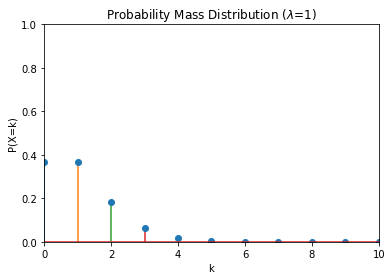
\includegraphics[scale=0.7]{lambda=1.png}
\end{figure}
\end{frame}
\subsection{PMF}
\begin{frame}
\frametitle{PMF Graphs}
\begin{figure}
    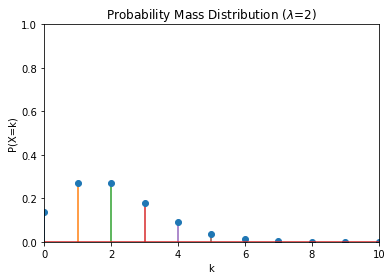
\includegraphics[scale=0.7]{lambda=2.png}
\end{figure}
\end{frame}
\subsection{PMF}
\begin{frame}
\frametitle{PMF Graphs}
\begin{figure}
    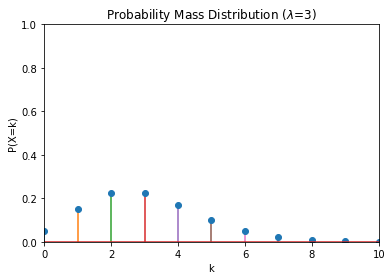
\includegraphics[scale=0.7]{lambda=3.png}
\end{figure}
\end{frame}
\subsection{PMF}
\begin{frame}
\frametitle{PMF Graphs}
\begin{figure}
    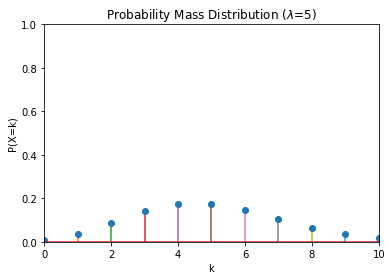
\includegraphics[scale=0.7]{lambda=5.png}
\end{figure}
\end{frame}
\begin{frame}
\frametitle{Cumulative Distribution Function}
Cumulative Distribution Function(CDF) is given by
\begin{align}
    F_X(k)&=\pr{X\le k}\\
    &=\sum_{n=0}^{n=k}\pr{X=n}
\end{align}
\end{frame}
\begin{frame}
\frametitle{CDF Graph}
\begin{figure}
    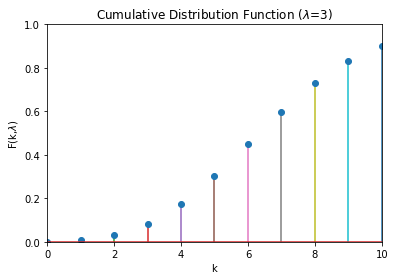
\includegraphics[scale=0.7]{cdf.png}
\end{figure}
\end{frame}
\begin{frame}
\frametitle{Example Question}
\begin{block}{Question}
Suppose that astronomers estimate that large meteorites (above a certain size) hit the earth on average thrice every 100 years and that the number of meteorite hits follows a Poisson distribution. What is the probability of  2 meteorite hits in the next 50 years?
\end{block}
\end{frame}
\begin{frame}
\frametitle{Solution}
\begin{block}{Solution}
Rate of meteors hitting is 3 per 100 years.\\
\begin{align}
    rate(r)=\frac{3}{100}
\end{align}
So, for 50 years, 
\begin{align}
    \lambda=r\cdot t=\frac{3}{100}\cdot 50=\frac{3}{2}=1.5
\end{align}
We have to find the probability of 2 meteors hitting in the next 50 years.\\
So, we have to find the value of $\pr{X=2}$ with $\lambda=1.5$\\
By putting the values of k=2 and $\lambda=1.5$ in \eqref{formula}
\begin{align}
    \pr{X=2}&=\frac{1.5^2\cdot e^{-1.5}}{2!}\\
    &=0.251
\end{align}
\end{block}
The PMF is as follows:
\end{frame}
\begin{frame}
\frametitle{PMF Graph}
\begin{figure}
    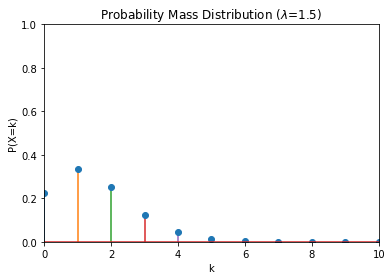
\includegraphics[scale=0.7]{example_pmf.png}
\end{figure}
\end{frame}
\end{document}